\documentclass[border=10pt]{standalone}
\usepackage{tikz}
\usetikzlibrary{arrows.meta}

\begin{document}
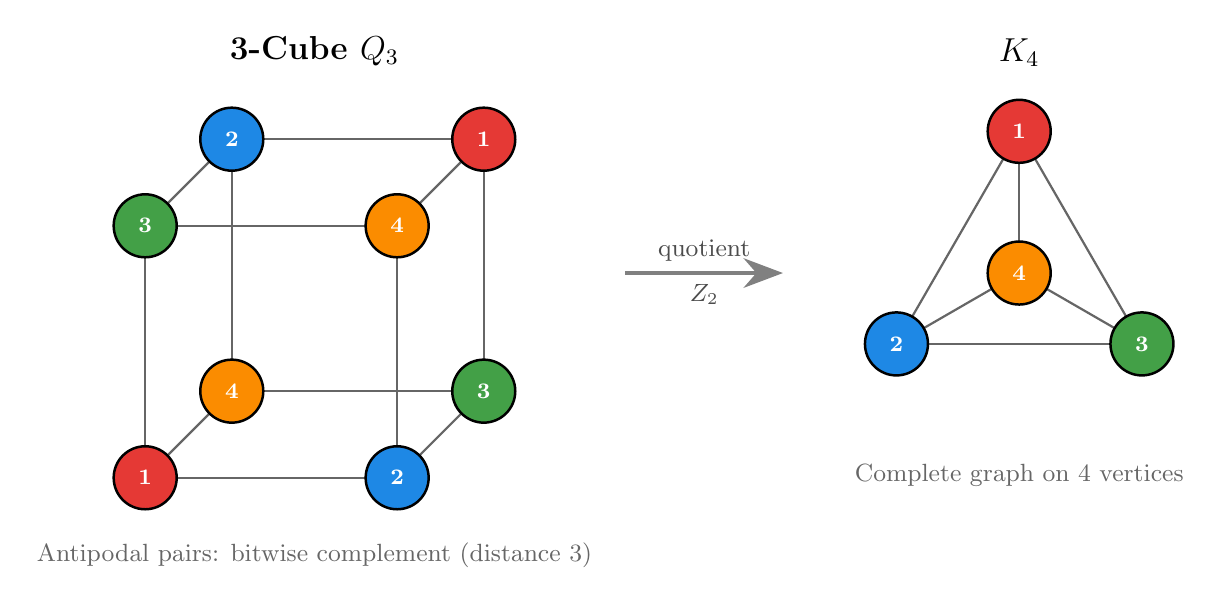
\begin{tikzpicture}[
    vtx/.style={circle, draw=black, line width=0.9pt, minimum size=8mm,
                inner sep=0pt, font=\footnotesize\bfseries},
    edge/.style={line width=0.8pt, black!60},
    quotarrow/.style={-{Stealth[length=5mm]}, line width=1.5pt, black!50}
]

% ============================================================
%  COLOR PALETTE (4 fibers)
% ============================================================
\definecolor{c1}{HTML}{E53935}   % red
\definecolor{c2}{HTML}{1E88E5}   % blue
\definecolor{c3}{HTML}{43A047}   % green
\definecolor{c4}{HTML}{FB8C00}   % orange

% ============================================================
%  3-CUBE — left side
% ============================================================
% Standard cube drawing: front face + back face + connecting edges
% Vertices labeled by binary: 0=000, 1=001, 2=010, 3=011, 4=100, 5=101, 6=110, 7=111
% Antipodal pairs (bitwise complement, distance 3):
%   {0,7} = {000,111}  →  fiber 1
%   {1,6} = {001,110}  →  fiber 2
%   {2,5} = {010,101}  →  fiber 3
%   {3,4} = {011,100}  →  fiber 4

% Front face (z=0): 0=000, 1=001, 2=010, 3=011
\coordinate (v0) at (-1.6, -1.6);
\coordinate (v1) at (1.6, -1.6);
\coordinate (v2) at (-1.6, 1.6);
\coordinate (v3) at (1.6, 1.6);

% Back face (z=1): 4=100, 5=101, 6=110, 7=111
\coordinate (v4) at (-0.5, -0.5);
\coordinate (v5) at (2.7, -0.5);
\coordinate (v6) at (-0.5, 2.7);
\coordinate (v7) at (2.7, 2.7);

% Draw back edges first (behind)
\draw[edge] (v4) -- (v5);
\draw[edge] (v4) -- (v6);
\draw[edge] (v5) -- (v7);
\draw[edge] (v6) -- (v7);

% Connecting edges
\draw[edge] (v0) -- (v4);
\draw[edge] (v1) -- (v5);
\draw[edge] (v2) -- (v6);
\draw[edge] (v3) -- (v7);

% Front edges
\draw[edge] (v0) -- (v1);
\draw[edge] (v0) -- (v2);
\draw[edge] (v1) -- (v3);
\draw[edge] (v2) -- (v3);

% Vertices with fiber colors
% Fiber 1: {0,7} red
\node[vtx, fill=c1, text=white] at (v0) {1};
\node[vtx, fill=c1, text=white] at (v7) {1};
% Fiber 2: {1,6} blue
\node[vtx, fill=c2, text=white] at (v1) {2};
\node[vtx, fill=c2, text=white] at (v6) {2};
% Fiber 3: {2,5} green
\node[vtx, fill=c3, text=white] at (v2) {3};
\node[vtx, fill=c3, text=white] at (v5) {3};
% Fiber 4: {3,4} orange
\node[vtx, fill=c4, text=white] at (v3) {4};
\node[vtx, fill=c4, text=white] at (v4) {4};

% Title
\node[font=\large\bfseries, anchor=south] at (0.55, 3.5) {3-Cube $Q_3$};
\node[font=\small, anchor=north, text=black!60] at (0.55, -2.3)
    {Antipodal pairs: bitwise complement (distance 3)};

% ============================================================
%  ARROW
% ============================================================
\draw[quotarrow] (4.5, 1.0) -- node[above, font=\small, text=black!70] {quotient}
                              node[below, font=\small, text=black!70] {$\mathbb{Z}_2$} (6.5, 1.0);

% ============================================================
%  K₄ — right side
% ============================================================
\begin{scope}[xshift=9.5cm, yshift=1cm]

\def\Rk{1.8}

% Vertices at corners of a regular tetrahedron projection
\coordinate (k1) at (90:\Rk);
\coordinate (k2) at (210:\Rk);
\coordinate (k3) at (330:\Rk);
\coordinate (k4) at (0, 0);

% All 6 edges (complete graph)
\draw[edge] (k1) -- (k2);
\draw[edge] (k1) -- (k3);
\draw[edge] (k1) -- (k4);
\draw[edge] (k2) -- (k3);
\draw[edge] (k2) -- (k4);
\draw[edge] (k3) -- (k4);

% Vertices
\node[vtx, fill=c1, text=white] at (k1) {1};
\node[vtx, fill=c2, text=white] at (k2) {2};
\node[vtx, fill=c3, text=white] at (k3) {3};
\node[vtx, fill=c4, text=white] at (k4) {4};

% Title
\node[font=\large\bfseries, anchor=south] at (0, \Rk+0.7) {$K_4$};
\node[font=\small, anchor=north, text=black!60] at (0, -\Rk-0.5)
    {Complete graph on 4 vertices};

\end{scope}

\end{tikzpicture}
\end{document}
